\chapter{Compartmental and Stochastic Models}
\section{Deterministic Models}

\subsection{SIR Model}

In the SIR model the population is partitioned into three compartments susceptible, infected and recovered This is the basis for most epidemiological models \citep{m1925applications}. In building the model the number of individuals susceptible, infected and recovered is assumed to be differentiable over time.
The simple epidemic model is given by,
\begin{center}
\begin{align} \label{eqn4.1}
\frac{dS}{dt} &= -\beta SI,\\
 \frac{dI}{dt} &=\beta S I - \gamma  I, \\
 \frac{dR}{dt} &= \gamma  I.
\end{align}
\end{center}

$N = S + I + R.$
The model is based on the assumption that susceptible individuals become infected at a rate $\beta$ proportional to the number of people infected and susceptible at time $t$ and infected people recover at $\gamma$ rate. The reciprocal $\frac{1}{\gamma}$ is referred to as the average infectious period. Another assumption in this model is that the population remains constant, thus it does not take int account the demographic changes of the population. Figure \ref{fig 4.1} shows the compartmental diagram for an SIR model without demographic dynamics.
\begin{figure}[h!]
\centering
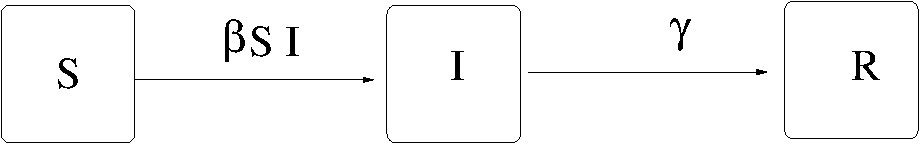
\includegraphics[scale=0.5]{images/sir.jpg} 
\caption{SIR compartmental diagram}\label{fig 4.1}
\end{figure}



\subsection{Model Analysis}
We determine the equilibrium and the stability of \ref{eqn4.1}, but since $N =S + I + R$ knowing $S$ and $I$ implies that we can solve for  $R$. Hence our system of equations can be reduced to 
\begin{align}
\frac{dS}{dt} &=-\beta SI. \label{eqn4.11} \\
 \frac{dI}{dt} &= \beta S I - \gamma  I \label{eqn4.22}.
\end{align}
 With $S(0) >0$, $I(0) > 0$ and $R(0) =0$ as the initial conditions for the model.
 We now calculate the disease free equilibrium and endemic equilibrium by equating equations \ref{eqn4.11} and \ref{eqn4.22} to zero then solving them. Despite its extreme simplicity, this model equation \ref{eqn4.1} cannot be solved explicitly. That is, we cannot obtain an exact analytical expression for the dynamics of S and I
though time, instead the model has to be solved numerically.

The equation \ref{eqn4.11} gives two import insights in understanding the spread of disease and has since been used in infectious disease modelling for a long time.

\subsection{Threshold Phenomenon} 
It is important to determine whether the infection will result in an epidemic or not and what are the determining factors. Consider the initial stage after $I (0) $ individuals have been infected in a population with $S (0) $ susceptible. Equation \ref{eqn4.22} can be rewritten as,
\begin{equation} 
\frac{dI}{dt} = I \left(\beta S -\gamma \right)\label{4.14}
\end{equation}
In equation \ref{4.14} if the initial susceptible (S(0)) is less than $\frac{\gamma}{\beta}$, then $\frac{dI}{dt} < 0 $. This means that there will be no epidemic in this case.

This result was coined by \cite{m1925applications} and  is refereed to as the threshold phenomenon. The initial S(0) must exceed the threshold $\frac{\gamma}{\beta}$ for an epidemic occur. In  other words the relative removal rate $\frac{\gamma}{\beta}$ must be small enough to allow the occurrence  of the epidemic.
 
 The reciprocal of the of relative removal rate is called the basic reproductive ratio and is one of the most important quantities in epidemiology. The basic reproduction ratio is defined as the average number of secondary cases arising from an average primary case in an entirely susceptible population. It measures measures the maximum reproductive potential for an infection. For the our SIR model in equation \ref{eqn4.1} it is given by:

\begin{equation}
R_0 = \frac{\beta}{\gamma}\label{eqn 4.15}
\end{equation}
 
For initial susceptible $S(0) = 1$, if $R_0 >1$ then there will be an outbreak and if $R_0<1$ the will be no outbreak. It can be noted that every disease has a different $R_0 $ value and also depending on the population's contact pattern the $R_0$ value will differ.

 \subsection{Epidemic Burnout}
 The threshold phenomena gives a description of what happens in the initial stages after introduction of an infection. Another important quantity we get from the SIR model is the long term state of the infection. From they system in equation \ref{eqn4.1} we take
 
 \begin{align}
 \frac{dS}{dt} &= -\beta S I \label{4.16}
 \\ \frac{dR}{dt}& = \gamma I \label{4.17}
\intertext{  dividing  equation \ref{4.14} by equation \ref{4.17} we get } \nonumber
\\ \frac{dS}{dR}& = \frac{-\beta S}{\gamma}
= - R_0 S \label{4.19}
 \end{align}
 Integrating equation \ref{4.19} with respect to R, we get; 
 
 \begin{align}
 \int{\dfrac{dS}{S}} &= -\int{ R_o dR}
 \\ ln S &= -R_0 R + k
 \\ e^{ln S} &= e^{-R_0 R + k}
 \\  S(t) &= e^{-R_0 R(t)} e^{k}
 \intertext {assuming R(0) = 0} \nonumber
 \\ S(t) = S(0)e^{-R_0 R(t)} \label{eqn 4.1.13}
 \end{align}
 
 Hence, as the epidemic develops, the number of susceptibles reduce. The numbered of recovered does not start increasing immediately because of infectious period, but eventually it does. Their number of susceptibility in the population will always be above zero as can be seen in equation \ref{eqn 4.1.13}.
 
From equation \ref{eqn 4.1.13}, $s(t) \geq e^{-R_o}$ since $R(t) <1$. Thus, there will always be a proportion of susceptibles in the population.  The epidemic burnout gives the intuitive idea that the chain of transmission eventually breaks due to the decline in infectives not due to lack of susceptibles \citep{haran2009introduction}.
 
 \subsection{Disease free equilibrium}Adding demographic parameters to \ref{eqn4.1} we get a new system of equations. That is, adding a parameter for birth rate and death rate, hence the population is no longer closed in this case.
 
 \begin{align}
 \dfrac{dS}{dt}& = \mu - \beta S I - \mu S \label{1}
 \\ \dfrac{dI}{dt}&= \beta SI - \gamma I -\mu I  \label{2}
 \\ \dfrac{dR}{dt} &= \gamma I - \mu R \label{3}
 \end{align}
 
 Using the same procedure we used to get the equation \ref{eqn 4.15} it can be shown that the $R_0$ for this model is \begin{equation}
R_0 = \frac{\beta}{\mu + \gamma} \label{eqn 4.2.17}
\end{equation}
 
 Now we calculate the equilibria  of the model by setting  equation \ref{1}, \ref{2} and \ref{3} to zero, that is $\dfrac{dS}{dt}= \dfrac{dI}{dt}= \dfrac{dR}{dt}= 0$ and denote by $S^*, I^*$ and $R^*$  values of  S, I and R that satisfy this condition. 
 From equation \ref{1} we get
 \begin{align}
  \mu -\beta SI - \mu S = 0 
  \\ \mu - S (\beta I + \mu ) = 0
  \\ S = \dfrac{\mu}{\beta I + \mu}
  \end{align}
 It can be shown that $S^* I^* R^* = (1,0,0)$ is the epidemic free equilibrium.
 
  To establish the endemic equilibrium , we factorize $I$ in  equation \ref{2} and  we get,
 \begin{align}
I (\beta S -(\gamma+ \mu)) = 0
 \intertext {thus we get}
 I = 0 \rightarrow S = \frac{\gamma+ \mu}{\beta}
 \end{align}
 Therefore, $I^* = 0$ and $S^* = \frac{\gamma+ \mu}{\beta}$, but since $I^* = 0$ is a disease free equilibrium. We concentrate on $S^* = \frac{\gamma + \mu}{ \beta} = \frac{1}{R_0} $ see \ref{eqn 4.2.17}
 
 Now, we take $I \neq  0 $ and solve \eqref{3}. Since $S+R+I =1$
 \begin{align}
 \gamma I - \mu (1 -S -I) = 0
 \\ \gamma I - \mu I -\mu (1-S) = 0
 \\ I = \frac{\mu}{\beta} R_0 \left( 1- \frac{1}{R_0} \right)
 \\ I = \dfrac{\mu}{\beta} (R_0 -1) 
 \end{align}
 
 Thus the endemic equilibrium point $( S^*,I^*,R^*)$ is 
 $\left( \frac{1}{R_0}, \frac{\mu}{\beta} (R_0 -1), 1 -  \frac{1}{R_0} \frac{\mu}{\beta} (R_0 -1) - \frac{1}{R_0} \right)$
 
 
  \subsection{Stability of the Model}
 Once an outbreak occurs, its important to understand the long term behaviour of the outbreak and finding the stability of the model gives an insight on this. In other words, calculating the stability of the model is establishing at which point the epidemic burn out will occur.
 \subsection{SEIR Model}
The susceptible, exposed, infected and recovered models add a new comportment to the previously discussed SIR Model. The earlier models assume that once a person is infected, they become infectious immediately. In this model an assumption is made that once a person is infected there is an intermediate stage between the time of infection and when they become infectious, this may be refereed to as the latent or incubation period of the infection. The system of equations will be;

\begin{align}
S'& = \mu -\beta S I - \mu S \label{5} \\
E' &= \beta S I - (\mu + \gamma) E  \label{6}\\
I' &= \gamma E - (\alpha + \mu I) \label{7}\\
R' &= \alpha I  - \mu R \label{8}
\end{align}
where $\beta$ is the rate at which susceptible individuals become infectious, $\gamma$ the rate at which infected individual become infection. The quantity $\frac{1}{\gamma}$ is called the latent period of the  infection and$\alpha$ is the recovery rate.
In this model the total number of infected individuals is given by $E +I$ and  we assume that our system is density dependant thus $S + E + I + R = 1$ and  that the population is constant implying that the birth rate ($\mu$)  = death rate $(\mu)$. Figure \ref{fig 4.2} shows the compartmental diagram of an SEIR model.
\begin{figure}[h!]
 
 \centering
 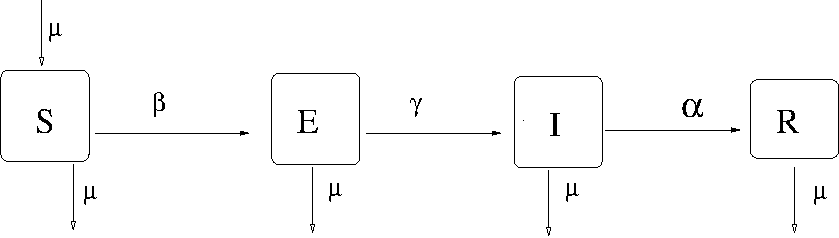
\includegraphics[scale=0.5]{images/seir.png}\label{fig 4.2}
 \caption{SEIR compartmental diagram}
 \end{figure}
  
 
Since $R = 1- S - E - I$
we can be drop equation \ref{8} from the system and  calculate equilibrium point by equating equations \ref{5} to \ref{7} to zero and solving the system of equations.

From equation \eqref{5} we get
$S = \dfrac{\mu}{\beta I - \mu}$ and from equation \ref{7} we get $I = \frac{\gamma E}{ (\alpha + \mu)}$ and from equation \ref{7} we get $ E = \dfrac{ \beta S I}{(\mu + \gamma)}$. Thus, for I = 0, E =0 and S = 1 hence, the disease free equilibrium of the system $S^*, E^*, I^* = (1,0,0)$.

 When $I^* \neq 0$ we find the disease pandemic equilibrium, which is given by
\begin{equation*}
S^*, E^*, I^*  = \left(\frac{(\alpha + \mu)(\gamma + \mu)}{\beta \gamma} , \frac{\alpha + \mu }{ \gamma} I^*, \frac{\mu}{\beta S*} \frac{\mu}{\beta} \right).
\end{equation*}

The reproductive number $R_0$  will be calculated using the new generation matrix method. Let F and V be non negative matrices,
\begin{equation}
F = \left[ \frac{\partial F_i (x^*)}{\partial j}\right]
\end{equation}  Where  $F_i (x^*)$ are the rates of new infections in compartment $i$ and 
\begin{equation}
 V = \left[\dfrac{\partial V_i(x*}{\partial j} \right]
\end{equation}
  Where $V_i (x^*)$ are the rates of transfer of infection from one compartment to another \citep{van2002reproduction}.
  $F =\left(\begin{array}{cc} 
0&0 \\ \beta&0
\end{array} \right)$ and $V = \left(\begin{array}{cc} \gamma + \mu & \gamma \\ 0& \alpha + \mu \end{array} \right)$


Therefore,
\begin{equation}\label{4.2.29}
FV^{-1} = \left(\begin{array}{cc} 
0&0 \\ \beta&0
\end{array} \right) \left(\begin{array}{cc}
\frac{1}{(\gamma + \mu)}&  \frac{-\gamma}{(\alpha +\mu)+ (\gamma + \mu)}\\ 0& \frac{1}{\alpha + \mu}  

\end{array} \right) = \left(\begin{array}{cc} 0&0 \\
\frac{\beta}{(\gamma + \mu)} &\frac{- \beta\gamma}{(\alpha +\mu)+ (\gamma + \mu)} 
\end{array}\right)
\end{equation}

The equation \ref{4.2.29} has eigenvalue values $\lambda_1$ , $\lambda_2$ as 0 and $\frac{- \beta\gamma}{(\alpha +\mu)+ (\gamma + \mu)}$ respectively.
 \begin{equation}
 R_0 = max {|\lambda_1| |\lambda_2|}
 \end{equation}
Thus the $R_0$ for the system will be $\frac{ \beta\gamma}{(\alpha +\mu)+ (\gamma + \mu)}$.

For the disease free equilibrium (1,0,0)is asymptotically stable if $R_0 < 1$ and unstable if $R_0 > 1$ \citep{van2002reproduction}. That is the solutions of the systems of equations \ref{5} \ref{7} move towards the disease free equilibrium when $R_0 < 1$.


%We examine the  behaviour of the stationary points by checking for their stability , we check the stability  of the system \ref{eqn 4.2.28}.
%
%
%
%Epidemiology compartmental models have been used for to model Infectious Diseases. Zika Virus can also be modelled using these compartmental models. A system of differential equations is used to model the dynamics of disease transmission.
%
%Zika Virus can be modelled by Susceptible , Exposed, Infectious and Recovered SEIR Model. Zika is mainly transferred by a vector(Mosquitoes). Thu the SEIR model takes into account the dynamics of pathogen transmission through vector.
%
%The compartment in this model are ; Susceptible denoted by $S_h(t)$ which is the number of people not carrying the pathogen but are prone to. Exposed denoted $E_h(t)$ This a number of people that have been exposed or have the pathogen but are not infectious. These include people that have had sex with a Zika infected person or people bitten by an infected mosquito but are yet to to exhibit symptoms and become infectious. Infectious denoted by $I_h(t)$ this compartment  comprises, people who are infected and infectious.That is they can transmit the disease to other people and they may or may not exhibit symptoms of being infected. Recovered denoted as $R_h(t)$, this compartment comprises of people that recover from the infectious or those that die or removed from the population. When some an infectious person is no longer infectious then then they are considered as recovered.
%
%Zika various is modelled with an SEIR model because one a person recovers from the infectious, studies have shown that they cannot be any reinfections. This was tested on monkeys who were cured of the infectious and Humans who have recovered from infectio\section{ Model Assumptions}
%
%
%
%The demographic variation in the number of people are not considered  and we also assume that the population among mosquitoes remains constant. This means the model does not take into death and birth among human beings. For the vectors death is assumed to be equal to birth hence the constant population. 
%
%All mosquitoes are assumed to be old to be adult mosquitoes, thus birth implies that an adult mosquito is added to into the proportion of mosquitoes.
%
%All humans have the the same probability of being infected. Either by mosquito bite or other means of  transmission. The period an organism (human or mosquito) stays in the Exposed compartment is called latent period and will be referred to as the incubation period.
%
%To model Zika virus on a random network, We take every person in the population as a vertex and when ever there is contact expected to result in the transmission of the  infection an edge is drown between the vertices. Therefore as property of a random graph, we assume that there is an equal probability of transmission between any given vertices in the graph. That is between any people in the population there is equal chance of disease transmission. This probability is used as the disease transmission rate in the SEIR model for Zika.
%
%\section{Compartmental Model}
%
%
%\section{Mathematical Model}%n \citep{posen2016epidemiology}.
%
%The vector ( Mosquitoes) also have a similar transmission of the pathogen. Though for the vector there are only three compartments. Susceptible denoted as $S_v$, this compartment comprises of a proportion of vectors that do not carry the pathogen hence can not infect anyone. The second compartment is the $E_V$ , which is a proportion of vectors that carry the pathogen but cannot infect or transmit to a human being. Lastly Infectious $I_v$ this is the proportion of vectors that can transmit the pathogens. It can be noted that since $S_v$,$E_v$ and $I_v$ are proportions, $ 0 \le S_v,E_v , I_v \le 1$ 
%

%
%The dynamical system of the transmission of Zika virus, is represented mathematically by the equations below.
%\begin{align}
%\begin{array}{lcl}  S'_h & = -&\beta_h S_h I_v  \\ E'_h & = & \beta_h S_h I_v - \alpha_h E_h  
%\\ I'_h &= &\alpha_h E_h - \gamma I_h 
%\\ R'_h &=& \gamma I_h 
%\\ 
%S'_v &=& \delta -\beta_v S_v \frac{I_h}{N} - \delta S_v
%\\ E'_v & = & \beta_v S_v \frac{I_h}{N} - (\delta + \alpha_v) E_v
%\\ I'_v & = &\alpha_v E_v - \delta I_V
% \end{array}
%\end{align}
%where :
%
%$\beta_h$  - Is the rate at which susceptible humans leave the susceptible compartment.
%
%$\alpha_h$ -  Is the rate at which exposed people become infectious.
%
%$\gamma$ - This is i the rate at which infectious individuals recover or get removed.
%
%$\delta$ -This is the birth rate of mosquitoes.
%
%$\alpha_v$ - This is the rate at which infected mosquitoes become infectious.
%
\section{Stochastic Models}
\subsection{ Stochastic SIR Model}
We will only consider an SIR model for the stochastic models. The total population $N(t) = S(t)  + I(t) + R(t)$ just as in deterministic models. Where 
\begin{align}
S(t), I(t), R(t) \in \left\lbrace 0,1,2,\dots , N \right\rbrace 
\end{align}
and $t \in \left\lbrace 0,\Delta t ,2 \Delta t, \dots \right\rbrace$. There are two independent discrete random variables  S, E and I because $R(t) = N(t) -S(t) -I(t)$. Therefore the stochastic process for the SIR model is a bivariate process $\left\lbrace S(t), I(t) \right \rbrace^{\inf}_{t =0}$ ha has a joint probability 

\begin{equation}
p_{(s+k,i+j),(s,i)}(\Delta t )= \Pr \left\lbrace( \Delta S ,\Delta I) = (k,j)\mid (S(t), I(t)) = (s,i) \right\rbrace
\end{equation}
where $\Delta S = S(t + \Delta t) - S(t)$. Hence the transition probability of the SIR model is a follows;
\begin{align}
p_{(s+k,i+j),(s,i)}(\Delta t )= \left\lbrace \begin{array}{ll}
 \beta i s / N \Delta t & (k,j) = (-1,1)
 \\ \gamma i \Delta t, & (k,j) = (0,-1)
 \\ b (N- s -i)\Delta t & (k,j) = (1,-1)
 \\ 1 - \beta i s/N \Delta t - \left[\gamma i +b(N-s) \right]n\Delta t ,& (k,j) =(0,0)
 \\ 0, otherwise
 \end{array} \right.
\end{align}
The time step $\Delta t$t must be chosen small enough such that each transition probabilities lie in the interval [0,1]. Applying the Markov property, the difference equation satisfied by the probability $p_{(s,i)} (t +\Delta t)$ can be expressed in terms of the transition probabilities.
\begin{align*}
p_{(s,i)} (t + \Delta t) &= p_{(s+1, i-1)}(t) (t) +\Delta t)rac{\beta}{N}(i -1)(s +1) \Delta t + p _{(s,i+1)} (t) \gamma (i +1) \Delta t \\ &+ p_{(s-1,i+1)}(t) b(i+1) \Delta t + p_{(s-1,i)}(t)b(N-s+1- i) \Delta t  \\&
+  {p_(s,i)}(t) \left(1 - \left[\dfrac{\beta}{N} is + \gamma i + b(N-s) \right] \Delta t\right)
\end{align*}

The difference equations can be written as in matrix form as 
\begin{equation*}
p_{(s,i)}(t + \Delta t) = P (\Delta t)p(t),
\end{equation*}
where $P(\Delta t)$ is the transition matrix and $p(t)$ is the probability distribution vector for the stochastic process.The state set is divided into two classes; the current and the transient.(N,0) is an adsorbing recurrent state while all other states are transient. The probability of an out break is given given as $1- \frac{1}{R_0}$ when $R_0 >1$ \citep{Brauer2017}.

One the main aspects in which deterministic and stochastic models differ is extinction. In deterministic SIR model an epidemic never goes to extinction in a limited time frame  because the number of infectives declines exponentially and only reaches zero at infinity.  In a deterministic framework an epidemic is said to go into extinction if it has a negative growth rate. Where as in the stochastic SIR model an epidemic is the  epidemic becomes extinct in a more direct sense, the number of infects can go to zero without waiting forever.